\documentclass{article}
\usepackage{geometry}[letter]
\usepackage{amsmath}
\usepackage{amssymb}
\usepackage{gensymb}
\usepackage{graphicx}

\title{Smart Lock Network}

\author{
  lockNET \\ \\
  Kenneth Ozdowy (kozdowy@umich.edu), Erik Liubakka (eliubakk@umich.edu) \\
  Cristian G\'{o}mez Peces (peces@umich.edu)
}
\date{}

\begin{document}

\maketitle

\section*{Changes from the First Proposal}

We have made the following changes to our design:


\subsection*{Hub}

On further research, we realized that a LoRa Gateway had every part of the Intel
Edison that we desired: web server capabilities, a cellular chip, and LoRa support. 

\subsection*{Lock}

Instead of using Arduinos to control the locks, we will be using the SmartFusion
boards instead. Not only do the SmartFusion boards give us more computability
power, they also allow us to add features otherwise impossible for the Arduino.
Firstly, we can implement our secure communication via RSA fully in hardware.
The change also allows more practical implementation of class material as opposed to
prebuilt Arduino libraries.

The locks themselves, instead of being regular door locks, will be simulated as
cabinet locks, with the servo turning a piece of metal that will prevent the
door from opening.

\section{Customer}
Our target market is people in communal living spaces such as houses or shared
apartments, and who are looking for greater control over the security of their
own rooms by using a central system with credentials to allow access through
doors as opposed to a simple key mechanism.

\section{Value}

The first benefit is the added security of the doors via two-factor
authentication. Each door can only be unlocked either via something on you (i.e.
NFC via a phone) or a part of you (i.e. fingerprint). This method
surpasses using a physical key because it can not be as easily duplicated or
lockpicked, and is also convenient as the odds of losing a key are much greater
than losing a smartphone or your fingerprints. The state of the door can also be
sent to the owner, so if they forgot to lock it they can just use their phone to
do so (or set up autolock functionality).

The second benefit is that there is more freedom in terms of access. Each door
can have both blacklists and whitelists to outright deny or accept people, and
if someone's on neither, they can request access remotely instead, much quicker
than waiting for them to come home. 

\section{Approach}

The top level design is of a central hub (a LoRa Gateway) with a number of nodes connected. The
hub is what allows users to communicate with the locks via a web interface. We
only want the hub to store what is necessary, acting as a control station while
each of the locks do most of the security part, making it much harder for
someone to spoof access rights. Each SmartFusion will have a hardware RSA
implementation in order to maintain secure communication (ensuring secure
communication on the hub side should be trivial).

When a scan occurs, the SmartFusion connected to the lock will compare the
credentials with its internal whitelist
and blacklist. If it's on the whitelist, the door will unlock. If it's on the
blacklist, not only will the door not unlock, but a record of the attempted
access is saved. If the credentials are on neither list, the SmartFusion will inform the hub,
which sends out a message to the lock's owner requesting approval. Upon
answer, the lock will unlock if approved. The request will also be recorded. If
the scan is via fingerprint, then only the prints already saved are allowed, and
no requests will be made if access is denied.

A similar messaging method will be used to make changes to the locks. In
order to allow equal ownership, if somebody wishes to change a common lock, they
submit a request for the change, and the others must approve it first before it
becomes implemented.

In case of power loss, the hub will have a backup power supply in order to
make users aware of the situation. A power-based interrupt will occur upon loss
of main power and the board will send out an SMS to all users.

NeoPixel LEDs would be used to provide visual feedback for the locks. There will
be different states for idle, waiting for response, access granted, access
denied, and an open door.

The following diagrams will showcase the control flow for the various operations
that the system will perform:

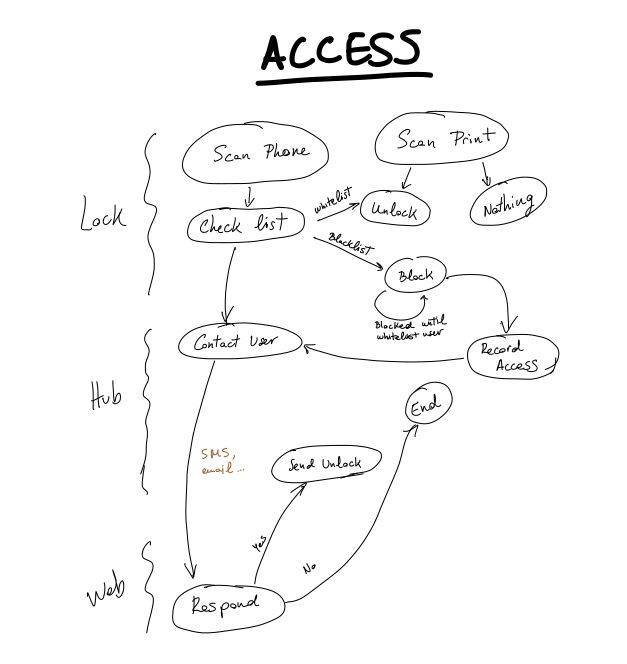
\includegraphics[scale=0.4]{access_graph.png}

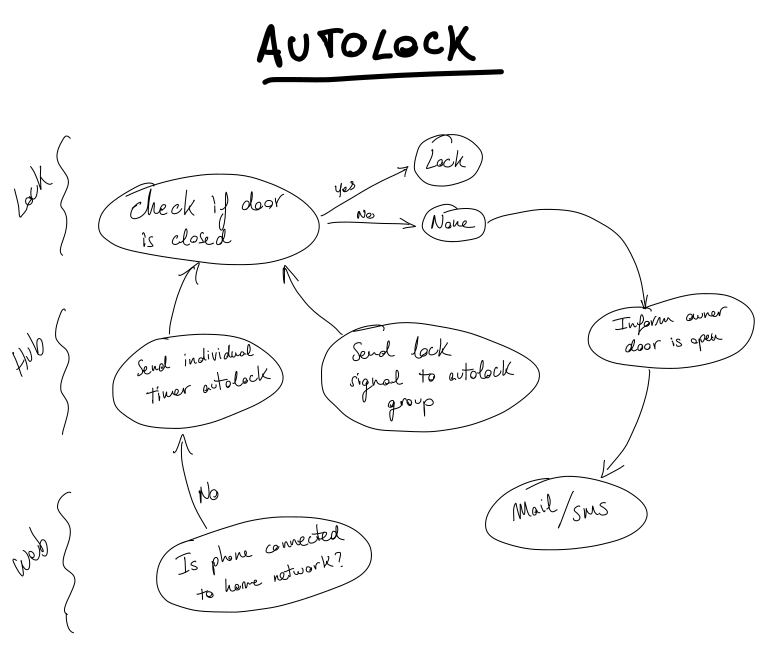
\includegraphics[scale=0.4]{autolock_graph.png}

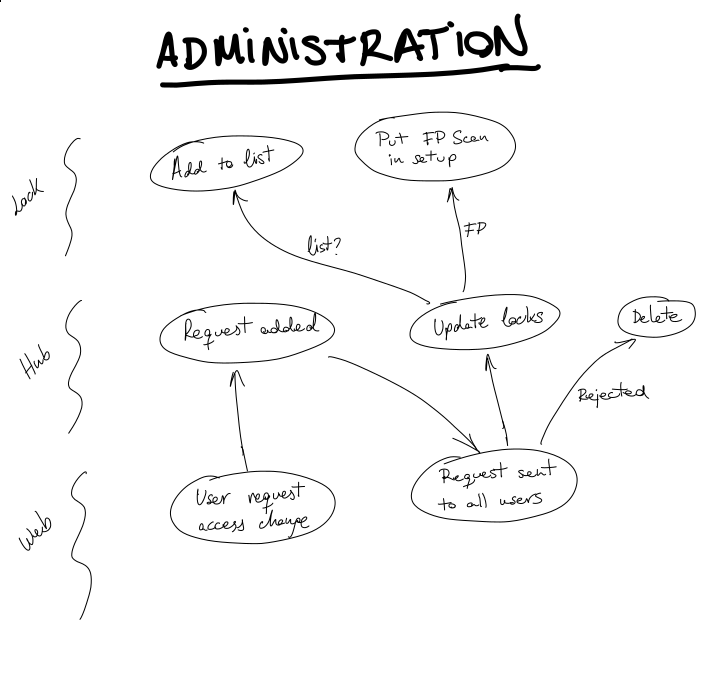
\includegraphics[scale=0.4]{admin_graph.png}

\section{Physical Components}


\subsection{Hub}

\noindent
Quantity: 1

\noindent
\begin{itemize}
\item \textbf{LG01 LoRa OpenWrt IoT Gateway} (Tindie)
  \item Panasonic LC-R121R3P 12V 1.3AH Sealed Lead Acid battery (Battery Clerk
    PN: AJC-D1.2S-J-0-142493)
    \end{itemize}


\subsection{Lock}

\noindent
Quantity: 2

\begin{itemize}
  \item \textbf{SmartFusion Board} (stock)
  \item Adafruit RFM95W LoRa Radio Transceiver Breakout - 868 or 915 MHz
    (Adafruit PID: 3072)
  \item Hitec HS-422 Servo (stock)
  \item Adafruit NeoPixel Digital RGB LED Strip (stock)
  \item KNACRO PN532 NFC Module 13.56MHz 3.3V Board (Amazon)
  \item Adafruit Industries LLC 375 Magnetic contact switch (Digi-Key PN: 1528-1907-ND)
  \item Portable USB Charger (stock)
\end{itemize}

\section{Potential Components}

\begin{itemize}
\item Fingerprint Scanner - TTL (GT-511C1R) (Sparkfun PID: SEN-13007)

The fingerprint scanner would be used as a failsafe in case the NFC reader was
not viable (either an issue with the scanner or with the NFC tag/phone). The
sensor itself communicates over UART and all of the heavy calculations are done
onboard, so it would be something completely separate from the credential
system that we have (which might be a positive, considering it's a failsafe).

\end{itemize}

\end{document}
